\documentclass{article}

\title{Dynamic metacommunity model to evaluate HPV strain interactions}
\author{Joe Mihaljevic}

\usepackage{geometry}
\geometry{legalpaper, portrait, margin=.75in}

\usepackage{Sweave}
\begin{document}
\Sconcordance{concordance:ReadMe.tex:ReadMe.Rnw:%
1 8 1 1 0 67 1 1 2 1 0 1 30 31 0 1 2 4 1 1 24 1 2 2 1 1 2 4 0 1 2 1 1 1 %
24 1 2 3 1 1 2 4 0 1 2 1 1 1 24 1 2 3 1 1 2 1 0 1 1 3 0 1 2 1 1 1 34 1 %
2 10 1}

\maketitle

\section*{Introduction}

The goal of this project is to create a dynamic, statistical, metacommunity model. Importantly, the model will allow for and estimate correlations among HPV strains so that hypotheses can be made as to which strains may ecologically interact via priority effects, facilitation, or competition.We will then apply this model to a data set of HPV co-infection dynamics across a large number of patients. The main novelties of this project are: (1) that we have a unique data set with many HPV strains across a large number of patients, and (2) that this is the first stastistical metacommunity model that estimates pair-wise correlations in the probabilities of colonization and persistence.

\section*{Model Specification}

HHere we will outline the dynamic, statistical metacommunity model. This model is based off of Dorazio et al. 2010, Ecology. Importantly, this model does not include the estimation of probability of detection, which corresponds in Dorazio 2010 to the probability of observing rare species. However, detection probability could later be incorporated in our model to reflect the sensitivity and specificity of HPV genotype testing.

Our data set consists of $K$ number of patients, who have been scored for the binomial occupancy of any of $I$ number of HPV strains over $T_{k}$ number of visits, where $T_{k}$ is allowed to vary among patients. Thus the data are of type $y_{ikt}$, which simply consists of a 0 or 1, depending on whether HPV strain $i$ was present in patient $k$ on visit $t$. 

First, we must estimate the initial occupancy probability for each HPV strain, which will then be used in a Markov Process to estimate how strain occupancy changes within and among individuals through time. 
$$y_{ik1} \sim Bern(\psi_{ik1})$$
$\psi_{ik1}$ estimates the probability that strain $i$ occupies patient $k$ at the patient's first visit. The occupancy probabilities for all subsequent visits depend upon the occupancy status of the previous visit, as follows:

$$y_{ik,t+1} \sim Bern(\psi_{ik,t+1})$$
$$\psi_{ik,t+1} = \phi_{ikt}\psi_{ikt} + \gamma_{ikt}(1-\psi_{ikt})$$

In this formulation, the likelihood of a patient retaining HPV strain $i$ from one visit to the next, depends upon the probability of strain $i$ being present at the previous visit, $\psi_{ikt}$, multiplied by the strain-, patient- and time-specific probability of persistence, $\phi_{ikt}$. This persistence probability can also be usefully thought of in terms of an extinction probability, $\xi_{ikt} = 1 - \phi_{ikt}$. Then, the probability that a patient $k$, who is previously uninfected with HPV strain $i$, becomes infected by strain $i$ at time $t+1$ is mediated by the colonization probability, $\gamma_{ikt}$.

\subsubsection*{Covariate effects and induced correlations}

One of our main goals is to determine how strain interactions might affect the ability of a given strain to colonize a new host or to persist in a host. However, we also want to control for the fact that certain strains may respond similarly to certain characteristics of the host environment. For example, if HPV strains A and B both favor young men, we would like to control for this common response when estimating how strain A might affect strain B's colonization probability. In order to account for strain responses to covariates and to simultaneosly estimate covariance among strains, we estimate colonization and persistence probabilities in the following way. For clarity, we will only present the model for persistence probability, although colonization probability is modeled in the exact same way. 

$$ logit(\phi_{ikt}) = \textbf{B}_{i}\textbf{X}_{k} + \textbf{B}^{k}_{i}\textbf{X}_{t[k]} $$

This model is a non-nested multi-level model, because patients have variable numbers of visits and some covariates are measured at the patient level and are static throughout the experiment, while other covariates are dynamic through time. Importantly, the structure of the data makes it easy to incorporate time-varying covariates in this framework, as the full set of covariates are measured at each visit, and time is indexed by visit number. In the above expression, $ \textbf{B}_{i} = (b_{0i}, b_{1i}, \dots, b_{qi})^{'} $ for $q$ number of covariate effects measured at the patient level that do not change across visits. Thus, $ \textbf{X}_{k} = (1, x_{1k}, x_{2k}, \dots, x_{qk}) $ holds the patient-level values of these covariates. We then incorporate a strain-specific, among-patient, random effect via by drawing the intercepts, $b_0$, from a multivariate normal distribution:

$$ b_0 \sim N(\mu_{\phi}, \Sigma_{b_{0}}), $$

where $\mu_{\phi}$ is the overall persistence probability given average covariate values (i.e. global average across strains), and $\Sigma_{b_{0}}$ is a covariance matrix, which accounts for among-patient correlations between strains' persistence probabilities:

$$ \Sigma_{b_{0}} = \left[
                \begin{array}{ccc}
                \sigma_{i}^2 & \dots & \rho_{i,I}\sigma_{i}\sigma_{I} \\
                \vdots & \ddots & \vdots \\
                \rho_{i,I}\sigma_{i}\sigma_{I} & \dots & \sigma_{I}^2
                \end{array}
                \right]
$$
Here $\sigma_{i}^2$ is the variance in persistence probability for strain $i$ across all patient samples. 

The next component of the model contains $ \textbf{B}^{k}_{i} = (b^k_{1i}, b^k_{1i}, \dots, b^k_{ri})^{'} $. These are strain-specific responses to covariates, $(1,...,r-1)$, that were measured at the patient-level. However, these covariates, $ \textbf{X}_{t[k]} = (1, x_{1t[k]}, x_{2t[k]}, \dots, x_{rt[k]}) $, are those covariates which were measured at the patient level and potentially have unique values for each patient visit $t$. Thus, we are able to also account for within-patient correlations between strains' persistence probabilites, similarly:

$$ b^k_1 \sim N(0, \Sigma_{b^k_{1}}), $$
where
$$ \Sigma_{b^k_{1}} = \left[
                \begin{array}{ccc}
                \sigma_{ik}^2 & \dots & \rho_{k_{i,I}}\sigma_{ik}\sigma_{Ik} \\
                \vdots & \ddots & \vdots \\
                \rho_{k_{i,I}}\sigma_{ik}\sigma_{Ik} & \dots & \sigma_{Ik}^2
                \end{array}
                \right]
$$
Here $\sigma_{ik}^2$ is the variance in persistence probability measured within patients for strain $i$ . 

Thus our model estimates both the among-patient and within-patient strain correlations in persistence and colonization probabilities. It is important to distinguish these among- and within-patient effects because the correlations among strains may be scale-dependent, with different processes leading to different patterns between the two scales (i.e. Simpson's paradox). For example, across all patients and visits, strains A and B may have positively correlated colonization probabilities resulting from the fact that both strain A and B tend to only be able to infect immuno-compromised individuals. However, within a patient, the strains' colonization probabilities might be negatively correlated if previous infection with strain A hinders the ability of strain B to superinfect. 

\section*{Simulation as proof of concept}

Here we will show that our model works in the sense that we can recover imposed parameters from simulated data. 

Our $sim_func()$ function simulates the occurrence of two HPV strains across a pre-determined number of patients and visits. The function allows us to manipulate many parameters including the strengths of within- and among-patient correlations in persistence and colonization. It also includes one patient-level and one visit-level covariate, the effects of which can be manipulated for each strain.

This is a simulated 'null' case in which we impose no correlations, and no covariate effects. 
\begin{Schunk}
\begin{Sinput}
> source("sim_func.R")
> null <- sim_func(n.pat = 100, #number of patients
+                  n.vis = 10,  #number of visits per patient (equal for each patient at this point)
+                  # Within and among host covariate effects for phi and gamma:
+                  bpat1g = 0, 
+                  bpat2g = 0,
+                  btime1g = 0,
+                  btime2g = 0,
+                  bpat1p = 0,
+                  bpat2p = 0,
+                  btime1p = 0,
+                  btime2p = 0,
+                  rag = 0, #rho.across.gamma
+                  rap = 0, #rho.across.phi
+                  rwg = 0, #rho.within.gamma
+                  rwp = 0, #rho.within.phi
+                  # sd across patients for each strain (phi and gamma):
+                  sap1 = 1, 
+                  sap2 = 1,
+                  sag1 = 1,
+                  sag2 = 1,
+                  # sd within patients for each strain (phi and gamma):
+                  swp1 = .4, 
+                  swp2 = .4,
+                  swg1 = .4,
+                  swg2 = .4,
+                  #Global probabilities:
+                  globphi = .5, 
+                  globgam = .5, 
+                  globpsi = .5)
\end{Sinput}
\end{Schunk}
This allows you to see all of the function's options, and you can see that the correlations (\emph{rag, rap, rwg, rwp}) are all set to zero.

Now we can view the correlations in $\gamma$ and $\phi$, and the induced correlations in $\psi$. The null example should have no such correlations.

\begin{center}
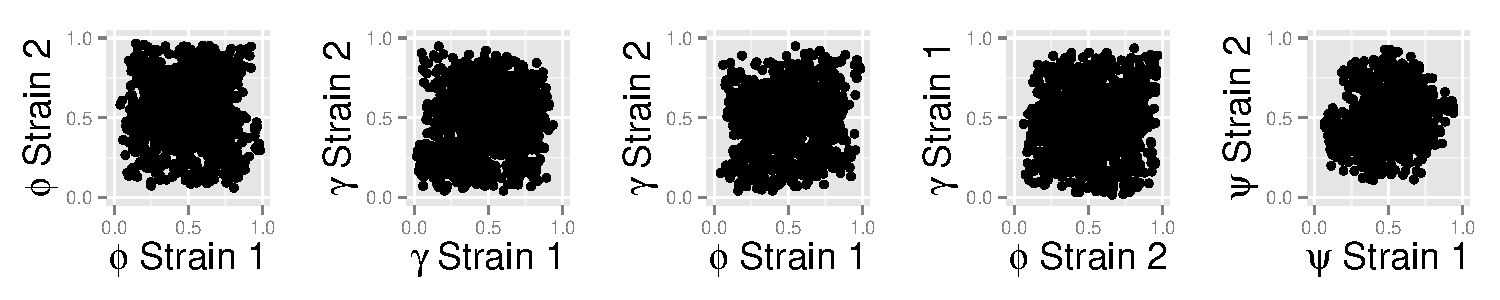
\includegraphics{ReadMe-002}
\end{center}

Let's assume strong correlations in among-patient persistence ($\phi$):
\begin{Schunk}
\begin{Sinput}
> corr.phi <- sim_func(rap = 0.9)
\end{Sinput}
\end{Schunk}

\begin{center}
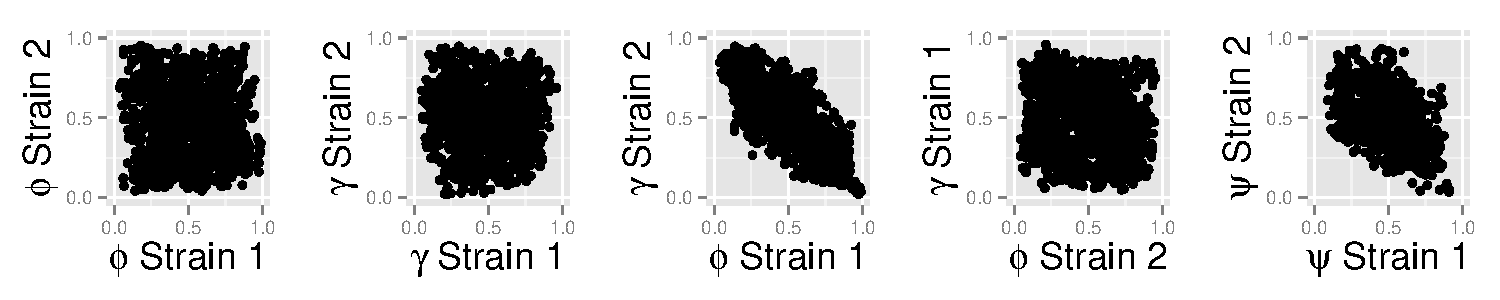
\includegraphics{ReadMe-004}
\end{center}

If we have high correlation in both $\phi$ and $\gamma$, then we see strong induced correlation in $\psi$.

\begin{Schunk}
\begin{Sinput}
> corr.both <- sim_func(rap = 0.9, rag = 0.9)
\end{Sinput}
\end{Schunk}

\begin{center}
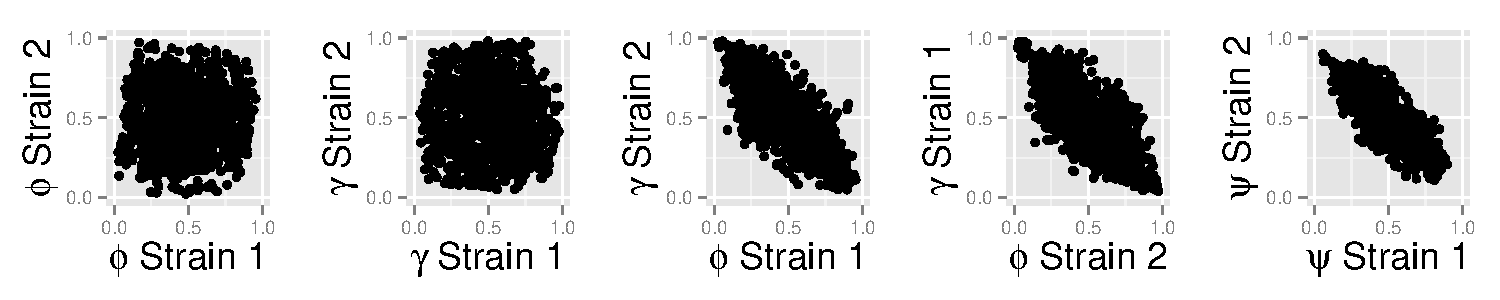
\includegraphics{ReadMe-006}
\end{center}

Let's compare if we have within and/or among-patient correlations in $\phi$ for example. I subsetted only 15 patients for clarity:

\begin{Schunk}
\begin{Sinput}
> among.phi <- sim_func(rap = 0.8)
> both.phi <- sim_func(rap = 0.8, rwp = -0.9)
\end{Sinput}
\end{Schunk}

\begin{center}
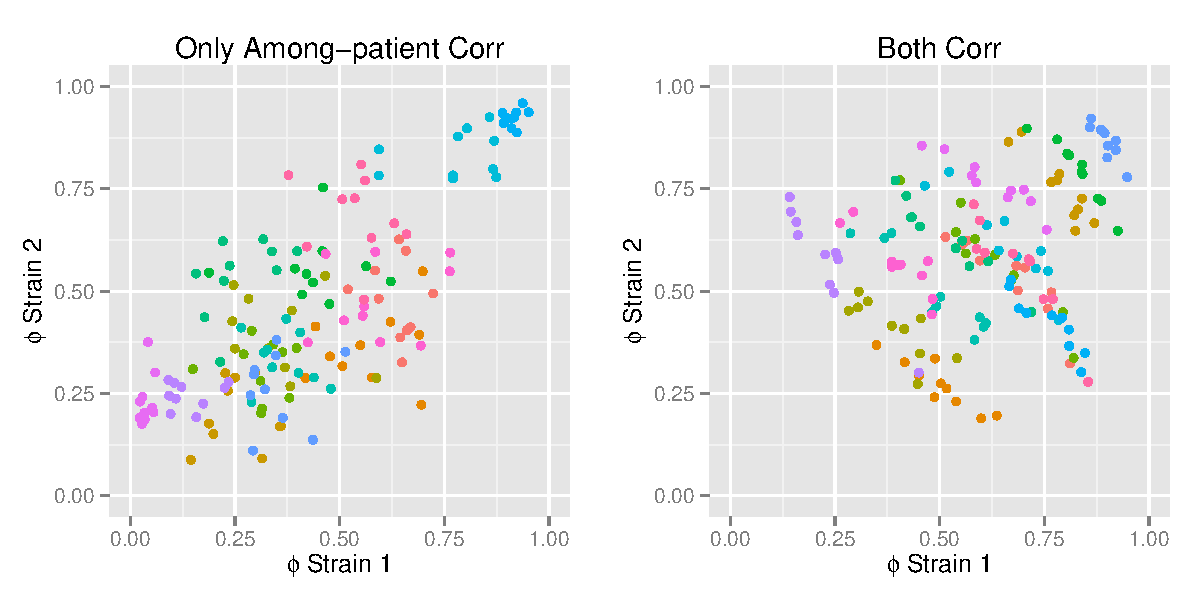
\includegraphics{ReadMe-008}
\end{center}

In the above figure, you can see that, with among-patient correlations, the $\phi$ values are grouped by patient (color), but there is random spread within the color grouping. However, when there is both within- and among-patient correlations, $\phi$ values are grouped by patient, but also the within-patient correlation is visible. You can alter the within and among correlations to be positive or negative and see what the figure looks like. For instance, you can generate Simpson's paradox with correlatinos of different sign. 

\end{document}






